% !TEX root = ../chem_ia.tex
\section{Background}
The stoichiometric reaction being studied in this investigation can be depicted as:
\[\ce{CH3COCH3_{(aq)} + I2_{(aq)} ->[HCl] CH3COCH2I_{(aq)} + HI_{(aq)}}\]
As the iodine is the limiting reagent, it is fully consumed to produce iodoacetone and hydrogen iodide so its brownish-red color slowly disappears from the reactant solution, allowing for the identification of the completion of the reaction~\parencite{other_literature_2, iodoacetone}. To determine the activation energy of this reaction, the time taken for completion was measured at various temperatures and the Arrhenius equation was then used. However, as the Arrhenius equation is dependent on the rate constant ($k$), it was first necessary to determine the rate law of the overall reaction.

Additionally, because of the slow nature of this reaction, the $HCl$ catalyst was used to provide an alternative pathway with a lower $E_a$. This allowed for a quicker rate, rendering the reaction feasible for the purpose of this investigation. The basic premise behind the significance of catalysts on lowering the $E_a$ and increasing the rate through kinetics can be seen in \cref{fig:background_1}.

% !TEX root = ../chem_ia.tex
\begin{figure}[h!]
     \centering
     \begin{subfigure}[t]{0.45\textwidth}
         \centering
         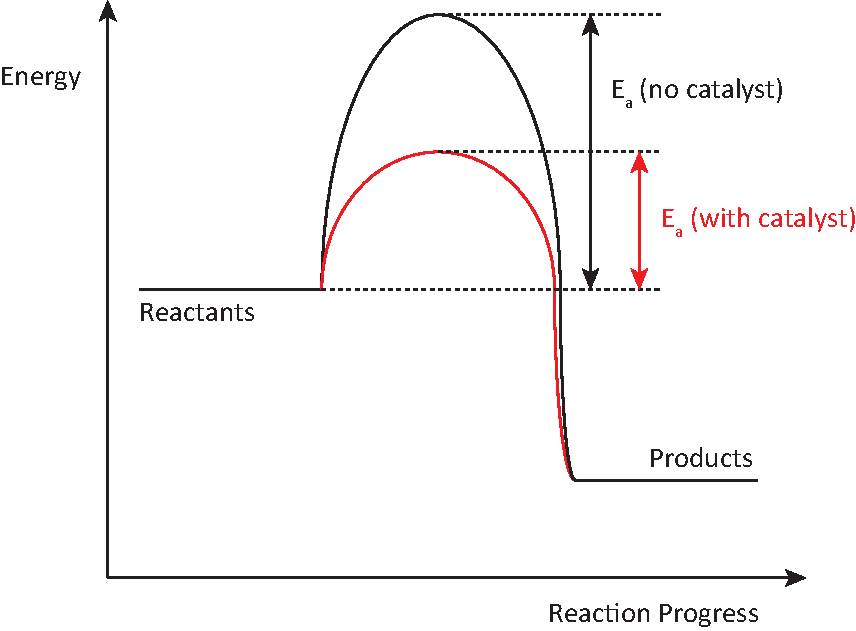
\includegraphics[width=\textwidth]{fig/images/catalyst_enthalpy.pdf}
         \caption{The catalyst provides an alternative pathway for the reaction with a lower $E_a$}
         \label{fig:catalyst-enthalpy}
     \end{subfigure}
        \hfill
     \begin{subfigure}[t]{0.45\textwidth}
         \centering
         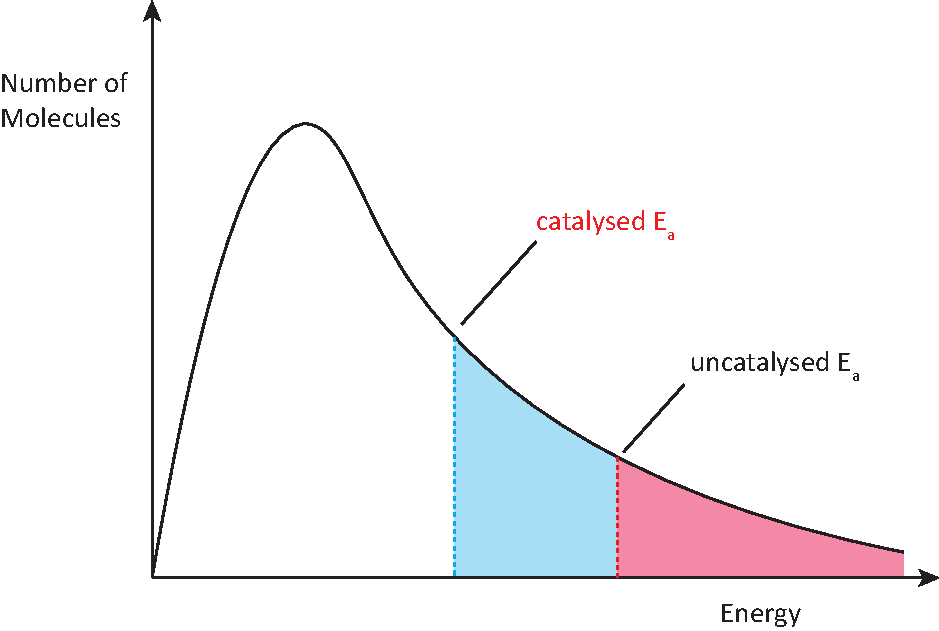
\includegraphics[width=\textwidth]{fig/images/catalyst_maxwell.pdf}
         \caption{The Maxwell Boltzmann Distribution shows how more molecules can then react as a larger proportion of molecules have sufficient energy ($>E_a$)~\parencite{Young_Freedman_Young_2020}.}
         \label{fig:catalyst-maxwell}
     \end{subfigure}
    \caption{Catalyst Function}
    \label{fig:background_1}
\end{figure}

\subsection{Rate Law and Reaction Mechanism}
Most reactions involving complex molecules/ions and catalysts rarely occur in a single step identical to the overall reaction, but instead can be further dissolved into multiple steps. This series of reactions is known as a reaction mechanism and plays an instrumental role in determining the rate of a reaction. Of these multiple steps, the slowest is referred to as the rate-determining step as it essentially dictates the rate of the overall reaction~\parencite{mechanism_information_ketone}. Multiple mechanisms are possible for this reaction (and thus have been proposed), but based on empirical evidence and the rate determined in this experiment, the most likely mechanism is shown in \cref{table:suggested_mechanism}.

\begin{table}[h!]
\centering
\begin{tabular}{m{6cm} m{10cm}} 
 \toprule
 Structural Depiction & Description \TBstrut\\
 \midrule
 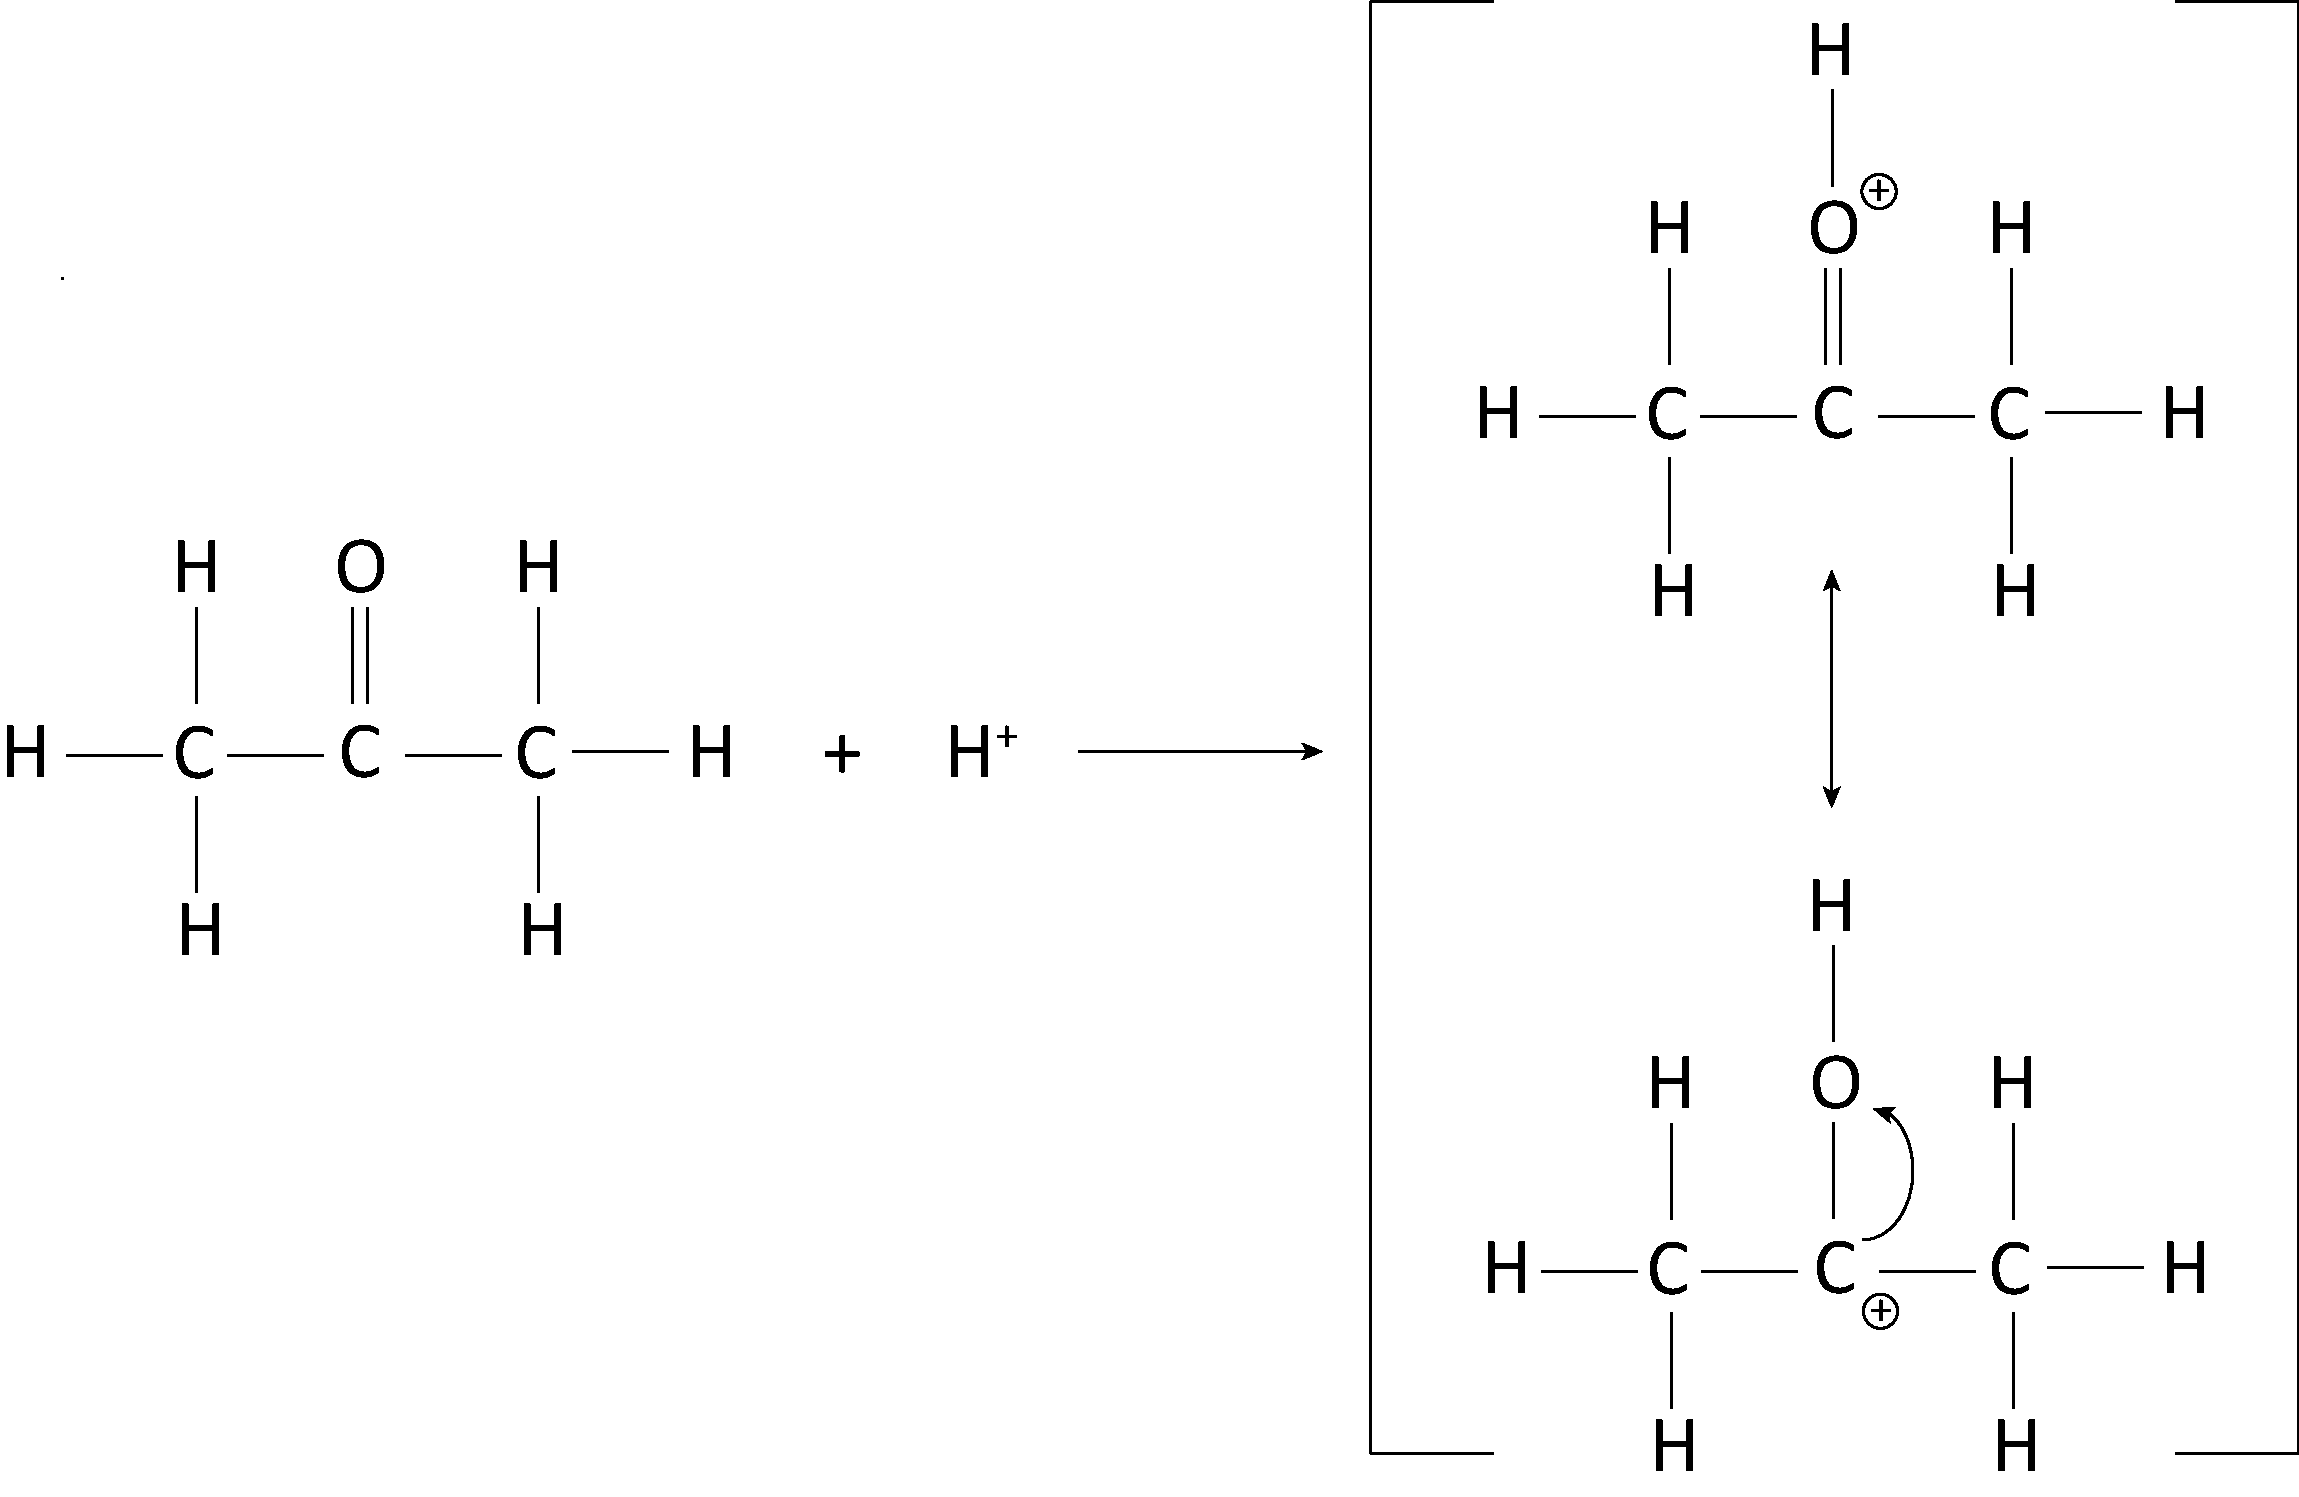
\includegraphics[width=.35\textwidth]{fig/images/mechanism/protonization.pdf} & Firstly, protonization of the carbonyl oxygen in acetone occurs as the acid donates its hydrogen ion. This process happens readily, as the highly polar double bond between carbon and oxygen makes the oxygen acquire a high partial negative charge ($\delta^-$). But, as the oxygen must donate both electrons for the electron pair (behave as a nucleophile), it acquires a positive charge. However, this structure is resonance stabilized, as if the more electronegative oxygen atom takes both electrons in its bond with carbon, the carbon will be left with the positive charge. \\
 \midrule
 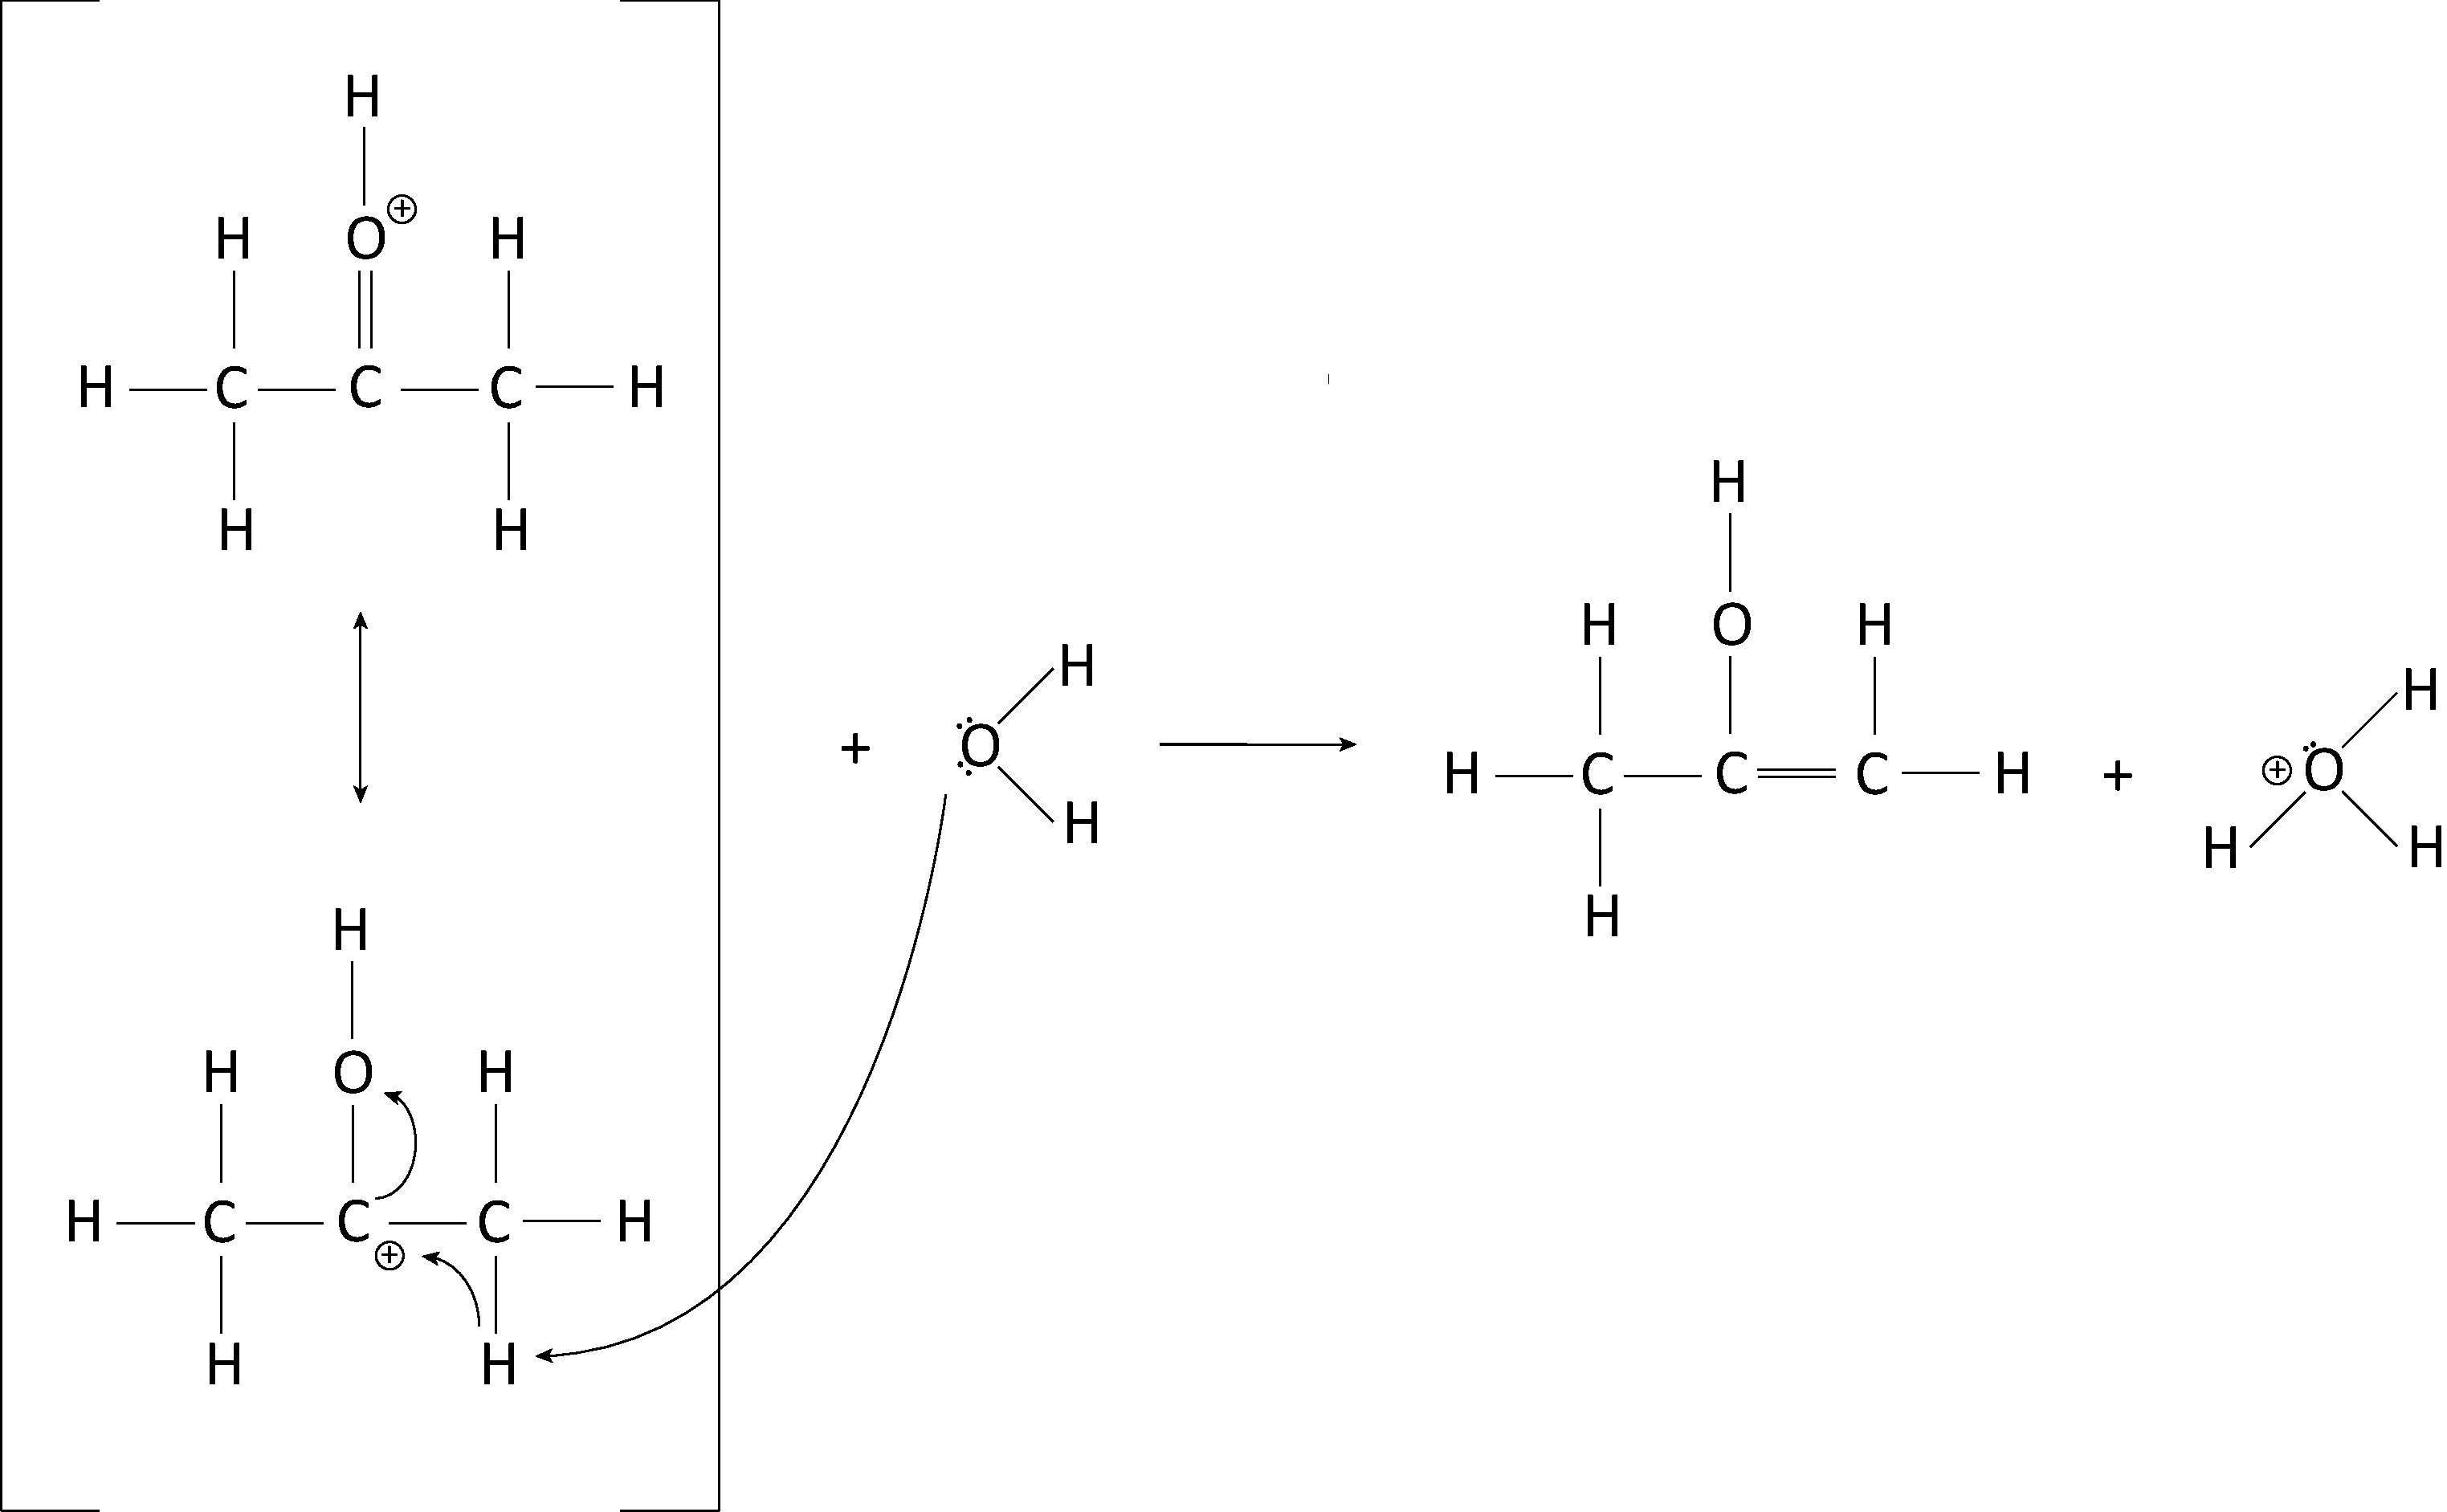
\includegraphics[width=.35\textwidth]{fig/images/mechanism/hydration.pdf} & Due to this polarization of the double bond, the $\alpha$-carbon also becomes more acidic, allowing for easier deprotonation. Thus, as the water molecule approaches, the highly electronegative oxygen with multiple lone pairs attracts a hydrogen molecule from the $\alpha$-carbon and behaves as a nucleophile. This produces hydronium ion (giving us back the acid catalyst) and the $\alpha$-carbon can form a double bond with the carbocation, resulting in an electrically neutral enol. These two steps together are referred to as enolization. \\
	\midrule
 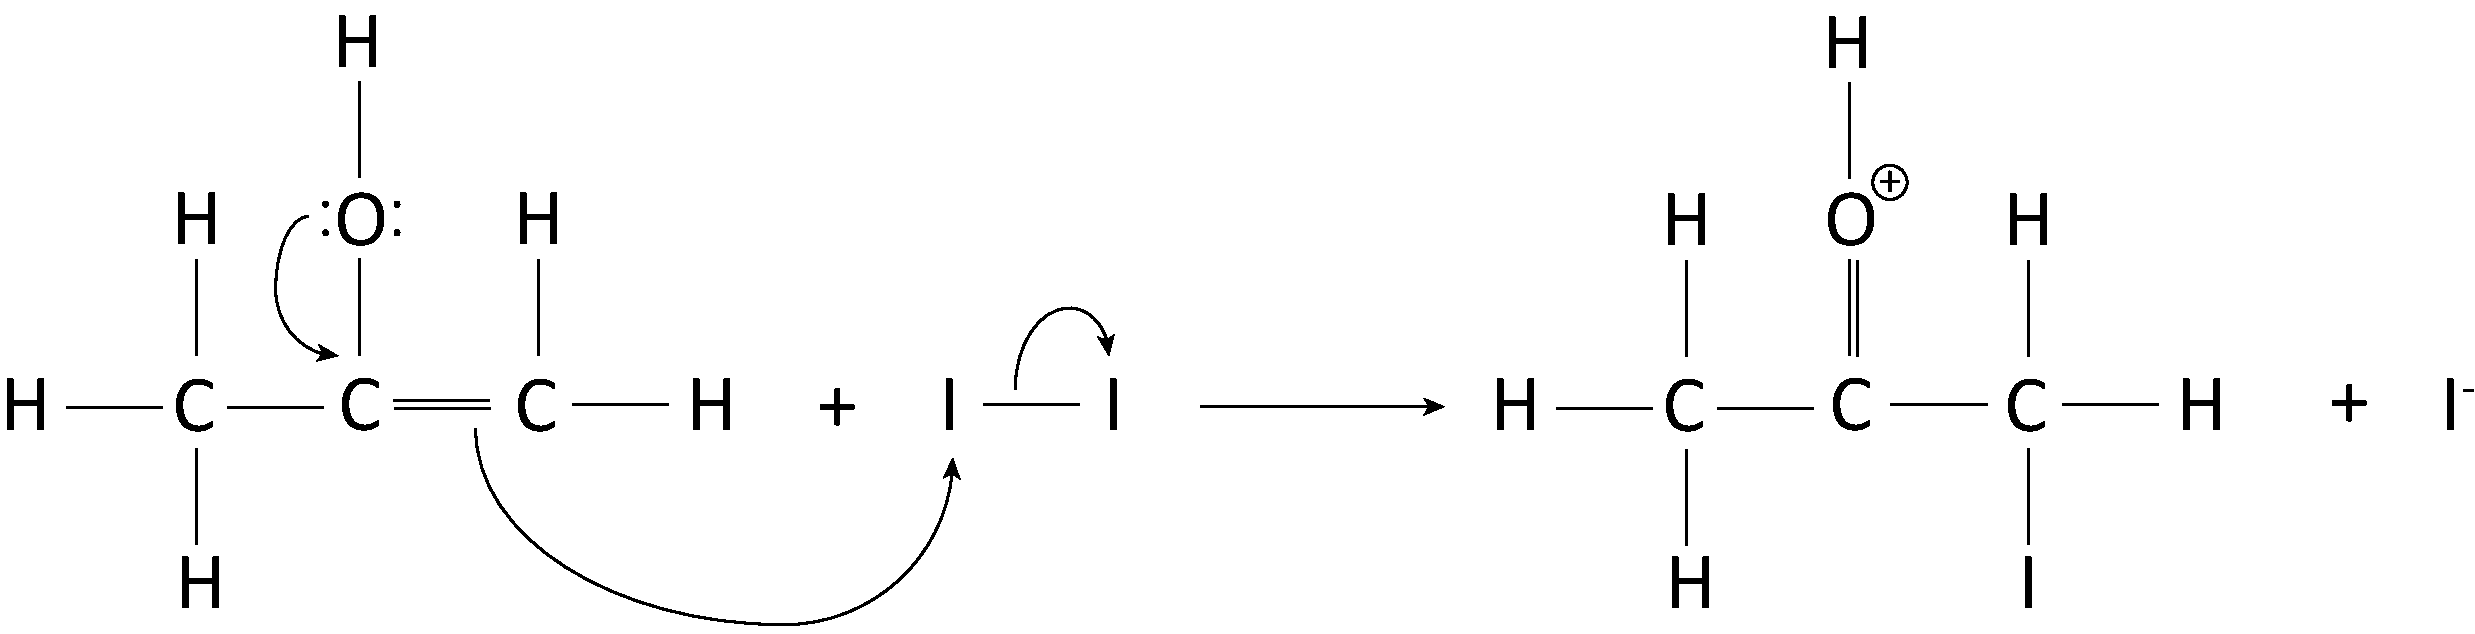
\includegraphics[width=.35\textwidth]{fig/images/mechanism/sn2.pdf} & 1 of the iodine atoms then behaves as an electrophile (as it is highly electronegative) and the enol becomes a nucleophile, facilitating a $S_N2$ attack and the heterolytical cleavage of the halogen molecule. The $\pi$-bond between the carbon atoms provides the electron pair for the positive iodine, and the oxygen is able to donate its lone pair, creating a dative bond to counteract the resulting positive charge on the carbon atom. This results in the halogenation of the $\alpha$-carbon and leaves a single iodine ion. \\
 \midrule
  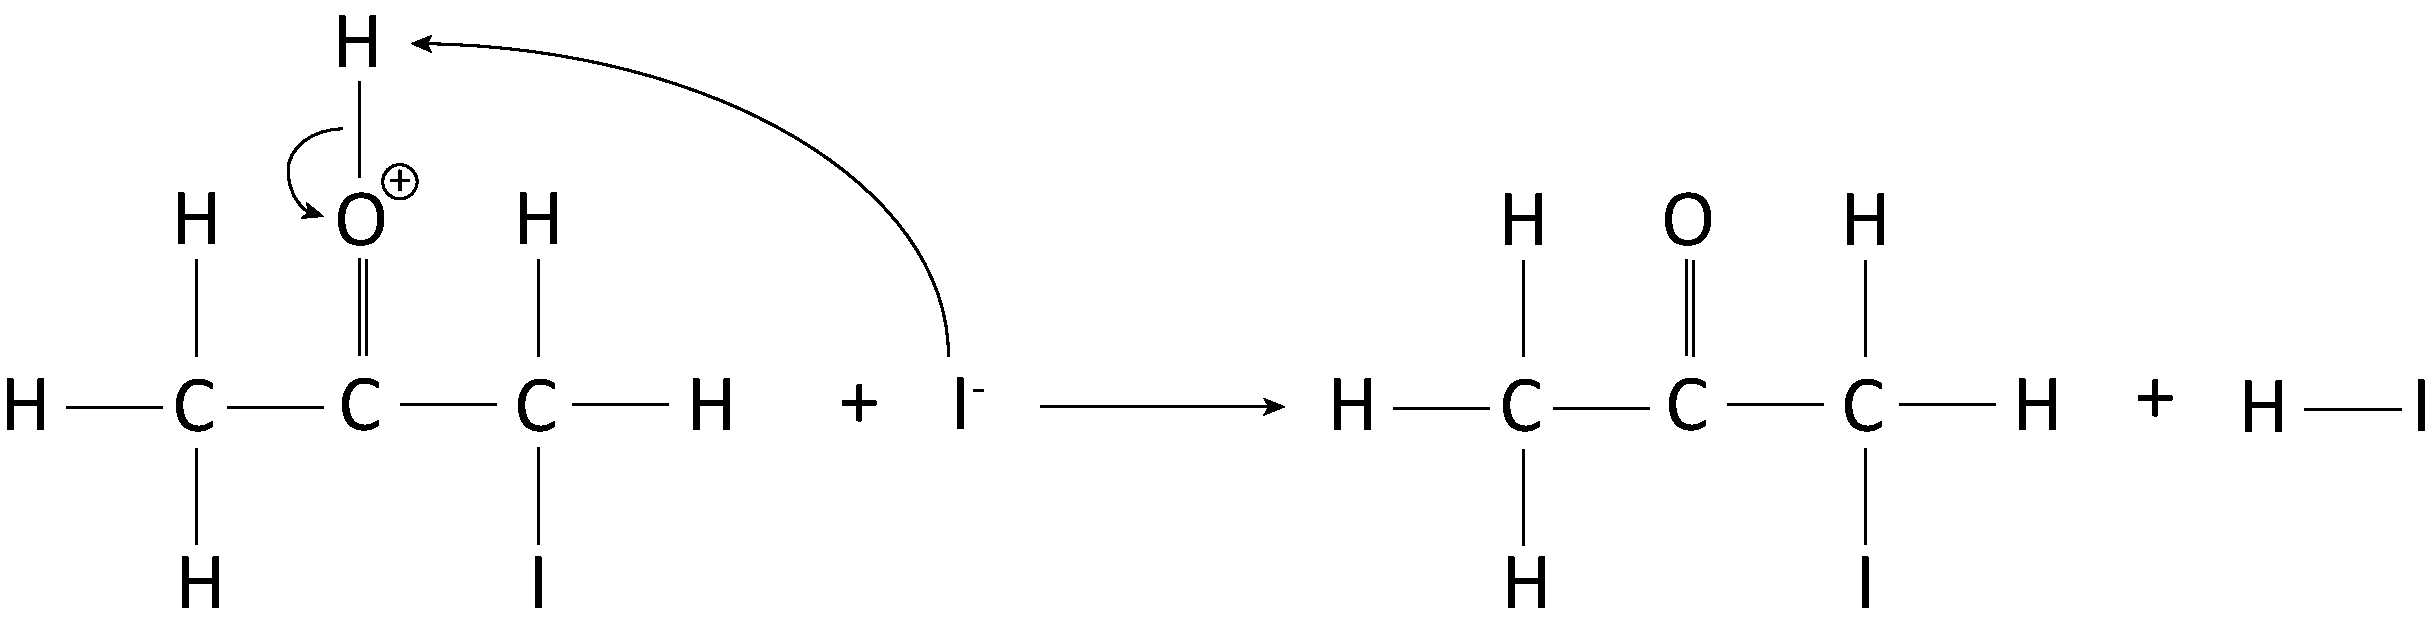
\includegraphics[width=.35\textwidth]{fig/images/mechanism/deprotonization.pdf} & Due to the resulting positive charge on the oxygen atom, the functional group becomes prime for deprotonization and facilitates the transfer of the hydrogen ion to the highly negative iodine ion. This leaves a double bond between the oxygen and carbon, providing a stable octet configuration for all species involved. \TBstrut\\
  \bottomrule
\end{tabular}
\caption{Proposed Mechanism}
\label{table:suggested_mechanism}
\end{table}

As ketones (specifically acetone) are extremely weak bases, the slowest step in this mechanism would be theorized as the initial one, where the acetone must acquire the donated proton from the acid catalyst. This process is slow even in the presence of a catalyst due to it not being enegetically favorable. Based on this empirical understanding (and the later confirmation via experimentation), this step is the rate-determining step~\parencite{alternative_approach_1}. As the speed of this step is dependent on the concentration of acetone and acid (not the halogen) which both have coefficients of 1, the overall rate law can be theorized as: $rate = k[CH_3COCH_3][HCl]$.

Although a catalyst is utilized for this reaction, it is still generally slow to complete at lower temperatures, making it difficult to perform many trials at lower temperatures. 

\subsection{Experimental Determination of Rate Law}

Although the empirical determination of the rate law can be suggested through the proposed mechanism above, it is still difficult to be fully confident in a rate law without experimental determination. Fortunately, this process is relatively straightforward and relies on basic mathematical principles. The general rate for any reaction can be expressed as a product of powers of the concentrations of all reactants and/or catalysts involved. Thus, for the iodination of acetone, the rate law must be:

\[rate = k[CH_3COCH_3]^p[HCl]^q[I_2]^r\]

where $p,q,r$ are integers greater than or equal to $0$. Additionally, $k$ is a constant for the reaction at a fixed temperature. Thus, by altering the concentration of individual reactants while keeping the remaining concentrations the same, different rates can be calculated and the results can be divided to determine the orders ($p,q,r$). For example, if we double the concentration of acetone while leaving the remaining concentrations untouched, we would have the result:

\[\frac{rate_2}{rate_1} = \frac{k[CH_3COCH_3]^p2^p[HCl]^q[I_2]^r}{k[CH_3COCH_3]^p[HCl]^q[I_2]^r} = 2^p\]

Then, by taking the logarithm (base 2) of both sides:

\[p = \log_2 \left(\frac{rate_2}{rate_1}\right)\]

This process can then be performed for the remaining reactants, allowing for the simple calculation of $p,q,r$ and the final determination/confirmation of the overall rate law~\parencite{intro_chemistry}.

\subsection{Determination of Activation Energy}
As mentioned previously, to determine the activation energy of a specific reaction, you must have the value of the rate constant $k$, which is temperature dependent. By finding/confirming the rate law of $rate = k[CH_3COCH_3][HCl]$, this process becomes straightforward. Because iodine is a limiting reactant, and acetone and acid are used in large excess quantities (keeping their concentration relatively stable), the rate is theorized to remain largely linear for the duration of the reaction~\parencite{other_literature_2}. Through this apparatus, the rate can then be defined as $\frac{\Delta [I_2]}{t}$, or the change in concentration of iodine over time. As the loss of color indicates reaction completion (and the total depletion of iodine), this simplifies to $\frac{[I_{2(initial)}]}{t}$. Then, through substitution and rearranging of the above rate equation, we see:

\[k = \frac{[I_{2(initial)}]}{t[CH_3COCH_3][HCl]}\]

This result allows us to experimentally determine the rate constant for various trials of this reaction. After calculating this rate constant at multiple temperatures, the Arrhenius Equation facilitates the determination of activation energy. The Arrhenius Equation highlights the dependence of the rate constant on the absolute temperature as~\parencite{arrhenius}:

\[k = Ae^{\frac{-E_a}{RT}}\]

where $A$ is the steric constant for each chemical reaction, $T$ is the absolute temperature (in Kelvin), and $R$ is the universal gas constant ($8.31 \frac{J}{K \cdot mol}$). Taking the natural log of this entire equation results in the following relationship:

\[\ln{k} = \left(\frac{-E_a}{R}\right)\frac{1}{T} + \ln{A}\]

Thus, a linear relationship exists between the natural logarithm of the rate constant ($\ln{k}$) and the inverse of the temperature($\frac{1}{T}$) with the gradient being $\frac{-E_a}{R}$. As $R$ is a known constant, a plot of the graph between these two variables can be used to find the slope of the line and thus the activation energy ($E_a$).